%&tex
\documentclass[12pt]{article}

\usepackage[a4paper,margin=1in]{geometry}
\usepackage{amsmath,amssymb}

\usepackage{graphicx}
\graphicspath{{""}}

\usepackage{cleveref}
\usepackage{subcaption}

\title{Potential Flow over Ellipse body}
\author{Ramkumar}

\begin{document}

\maketitle

\section{Problem Definition}
In this work, the potential flow over ellipse body is simulated using potential
flow theory. The code was made as a custom application in OpenFOAM v2206 and
the postprocessing is done using ParaView. The main aim of this work is to
introduce the OpenFOAM programming powers to the users.

\section{Governing equations}\label{eqnSection}
In this work, the potential flow elements containing a uniform flow, a source
and a sink positioned appropriately to form an ellipse body inside flowfield.
The main equation that is used to compute streamfunction \(\psi\) is given in
\Cref{psiEqn}.


\begin{align}
	\psi = V_{\infty} \cdot r \cdot sin(\theta) + \frac{\Lambda}{2\pi}\left(\theta_{sink} - \theta_{source} \right)  \label{psiEqn}
\end{align}

where,

\hspace{1cm}
\begin{tabular}{lcl}
	\(\displaystyle{V_{\infty}}\) & - & free stream velocity magnitude \\
	\(\displaystyle{\theta}\) & - & angle w.r.t. global origin \\
	\(\displaystyle{\theta_{sink}}\) & - & angle w.r.t. sink center \\
	\(\displaystyle{\theta_{source}}\) & - & angle w.r.t. source center \\
	\(\displaystyle{r}\) & - & radial distance w.r.t. global center \\
	\(\displaystyle{\Lambda}\) & - & source and sink's strength \\
\end{tabular} \newline

The velocity components in cartesian coordinates were calculated by taking gradient
of \(\displaystyle{\psi}\) field, as shown in \Cref{UxEqn,UyEqn}.
\begin{align}
	U_x &= \frac{\partial \psi}{\partial y} \label{UxEqn} \\
	U_y &= -\frac{\partial \psi}{\partial x} \label{UyEqn}
\end{align}\\

A rectangular mesh was made using \emph{blockMesh} utility in OpenFOAM and the cell
centers and boundary face centers in the mesh were used as the computation points
for streamfunction \(\phi\) and other variables. The radial distance \(r\)
and azimuthal distance \(\theta\) are calculated using the Equations
\ref{eqnR} and \ref{eqnTheta}, respectively.

\begin{align}
	r & = \sqrt{\Delta x^2 + \Delta y^2} \label{eqnR} \\
	\theta & = arctan2( \Delta y, \Delta x) \label{eqnTheta}
\end{align}\\

\section{Computation Methodology}
The steps followed in OpenFOAM to generate the semi-infinite body are given below.


\begin{enumerate}
	\item a new custom application was made in OpenFOAM v2206 and named as \emph{PotentialFlow\_ellipse} using command \emph{foamNewApp appName}.
	\item totally new 1 volScalarField and 1 volVectorField were created to store computed \(\displaystyle{\psi}\) and \(\displaystyle{U}\) using the equations mentioned in the Section \ref{eqnSection}.
	\item a loop over cells is created using which the field values for each cell is computed and a similar loop is created to go over boundary faces, then at the end of 2\textsuperscript{nd} loop the solution fields will be writen to the \emph{0} folder in the case directory.
\end{enumerate}

The result obtained using the OpenFOAM code is shown as a contour with streamlines that were made using \emph{ParaView}, in \Cref{fig:contour}.

\begin{figure}
	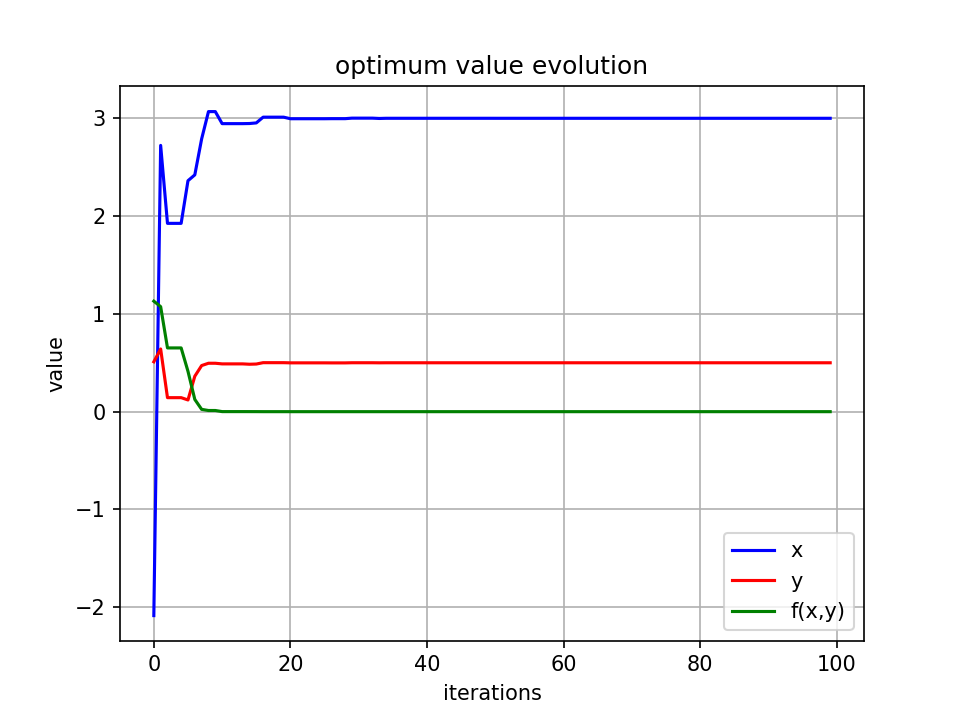
\includegraphics[scale=0.3]{../02_testCase/output.png}
	\caption{streamlines contour of semi-infinite body}
	\label{fig:contour}
\end{figure}

\pagebreak

\section{Instructions}
The instruction to generate/execute the files present in this work is given below.

\begin{enumerate}
	\item copy the contents of this entire root folder named \emph{02\_PotentialFlowOverEllipse} to a new directory.
	\item go into the subfolder named \emph{03\_OpenFOAMCode} which contains another sub-subfolder named \emph{PotentialFlow\_ellipse}, go into that using the terminal which is enabled with OpenFOAM environment.
	\item in the terminal, type \emph{wclean} and press enter, to clean any previous compilation files. Then type \emph{wmake} and press enter, this will compile the application.
	\item after compilation, cd to the directory named \emph{02\_testCase} and execute the command named \emph{PotentialFlow\_ellipse}. this should compute the field values and store them in the \emph{0} folder.
	\item after computation, use \emph{ParaView} for visualization of results.
\end{enumerate}

\end{document}
